\documentclass[11pt, addpoints, answers]{exam}

\usepackage[utf8]{inputenc}
\usepackage[T1]{fontenc}
\usepackage[margin  = 1in]{geometry}
\usepackage{amsmath, amscd, amssymb, amsthm, verbatim}
\usepackage{mathabx}
\usepackage{setspace}
\usepackage{float}
\usepackage{color}
\usepackage{graphicx}   
\usepackage[colorlinks=true]{hyperref}
\usepackage{tikz}

\usetikzlibrary{shapes,arrows}
%%%<
\usepackage{verbatim}
%%%>
\usetikzlibrary{automata,arrows,positioning,calc}

\usetikzlibrary{trees}

\shadedsolutions
\definecolor{SolutionColor}{RGB}{214,240,234}

% \usepackage{xcolor}
\usepackage{listings}

\lstset{language=R,
    basicstyle=\small\ttfamily,
    stringstyle=\color{black},
    otherkeywords={0,1,2,3,4,5,6,7,8,9},
    morekeywords={TRUE,FALSE},
    deletekeywords={data,frame,length,as,character},
    keywordstyle=\color{blue}
}

\newcommand{\bbC}{{\mathbb C}}
\newcommand{\R}{\mathbb{R}}            % real numbers
\newcommand{\bbR}{{\mathbb R}}
\newcommand{\Z}{\mathbb{Z}}            % integers
\newcommand{\bbZ}{{\mathbb Z}}
\newcommand{\bx}{\mathbf x}            % boldface x
\newcommand{\by}{\mathbf y}            % boldface y
\newcommand{\bz}{\mathbf z}            % boldface z
\newcommand{\bn}{\mathbf n}            % boldface n
\newcommand{\br}{\mathbf r}            % boldface r
\newcommand{\bc}{\mathbf c}            % boldface c
\newcommand{\be}{\mathbf e}            % boldface e
\newcommand{\bE}{\mathbb E}            % blackboard E
\newcommand{\bP}{\mathbb P}            % blackboard P

\newcommand{\ve}{\varepsilon}          % varepsilon
\newcommand{\avg}[1]{\left< #1 \right>} % for average
%\renewcommand{\vec}[1]{\mathbf{#1}} % bold vectors
\newcommand{\grad}{\nabla }
\newcommand{\lb}{\langle }
\newcommand{\rb}{\rangle }

\def\Bin{\operatorname{Bin}}
\def\Var{\operatorname{Var}}
\def\Geom{\operatorname{Geom}}
\def\Pois{\operatorname{Pois}}
\def\Exp{\operatorname{Exp}}
\def\Weibull{\operatorname{Weibull}}
\newcommand{\Ber}{\operatorname{Ber}}
\def\Unif{\operatorname{Unif}}
\def\No{\operatorname{N}}
\newcommand{\E}{\mathbb E}            % blackboard E
\def\th{\theta }            % theta shortcut
\def\V{\operatorname{Var}}
\def\Var{\operatorname{Var}}
\def\Cov{\operatorname{Cov}}
\def\Corr{\operatorname{Corr}}
\newcommand{\epsi}{\varepsilon}            % epsilon shortcut

\providecommand{\norm}[1]{\left\lVert#1\right\rVert} %norm
\providecommand{\abs}[1]{\left \lvert#1\right \rvert} %absolute value

\DeclareMathOperator{\lcm}{lcm}
\newcommand{\ds}{\displaystyle}	% displaystyle shortcut

% Distributions.
% \newcommand*{\UnifDist}{\mathsf{Unif}}
% \newcommand*{\ExpDist}{\mathsf{Exp}}
% \newcommand*{\DepExpDist}{\mathsf{DepExp}}
% \newcommand*{\GammaDist}{\mathsf{Gamma}}
% \newcommand*{\LognormalDist}{\mathsf{LogNorm}}
% \newcommand*{\WeibullDist}{\mathsf{Weib}}
% \newcommand*{\ParetoDist}{\mathsf{Par}}
% \newcommand*{\NormalDist}{\mathsf{Normal}}

% \newcommand*{\GeometricDist}{\mathsf{Geom}}
% \newcommand*{\NegBinomialDist}{\mathsf{NegBin}}
% \newcommand*{\BinomialDist}{\mathsf{Bin}}
% \newcommand*{\PoissonDist}{\mathsf{Poisson}}
\newcommand*{\Prob}{\mathbb{P}}
% \newcommand*{\Cov}{\mathsf{Cov}}


\def\semester{2023-2024}
\def\course{Modèle de Durée}
\def\title{\MakeUppercase{Examen final}}
\def\name{Pierre-O Goffard}
%\def\name{Professor Wildman}

\setlength\parindent{0pt}

\cellwidth{.35in} %sets the minimum width of the blank cells to length
\gradetablestretch{2.5}

%\bracketedpoints
%\pointsinmargin
%\pointsinrightmargin

\begin{document}


\runningheader{\course  \vspace*{.25in}}{}{\title \vspace*{.25in}}
%\runningheadrule
\runningfooter{}{Page \thepage\ of \numpages}{}

% \firstpageheader{Name:\enspace\hbox to 2.5in{\hrulefill}\\  \vspace*{2em} Section: (circle one) TR: 3-3:50 \textbar\, TR: 5-5:50 \textbar\,  TR: 6-6:50(Xu) \textbar\,  TR: 6-6:50 }{}{Perm \#: \enspace\hbox to 1.5in{\hrulefill}\\ \vspace*{2em} Score:\enspace\hbox to .6in{\hrulefill} $/$\numpoints}
\extraheadheight{.25in}

\hrulefill

\vspace*{1em}

% Heading
{\center \textsc{\Large\title}\\
	\vspace*{1em}
	\course -- \semester\\
	Pierre-O Goffard\\
}
\vspace*{1em}

\hrulefill

\vspace*{2em}

\noindent {\bf\em Instructions:} On éteint et on range son téléphone.
\begin{itemize}
	\item La calculatrice et les appareils éléctroniques ne sont pas autorisés.
	\item Vous devez justifier vos réponses de manière claire et concise.
	\item Vous devez écrire de la manière la plus lisible possible. Souligner ou encadrer votre réponse finale.
	\item \underline{Document autorisé:} Une feuille manuscrite recto-verso

\end{itemize}


\begin{center}
	\gradetable[h]
\end{center}

\smallskip

\begin{questions}
\question Le temps avant la défailance d'un composant électronique est modélisé via la variable aléatoire $T\sim\text{Lomax}(\alpha)$ dont la densité est donnée par 
$$
f(t) = \alpha(t+1)^{-\alpha-1}\mathbb{I}_{(0,\infty)}(t).
$$
\begin{parts}
\part[1] Donner la fonction de survie et la fonction de hasard de $T$.
\begin{solution}
$$
S(t) = (1+t)^{-\alpha}\text{ (0.5 point), et }h(t) = \alpha(1+t)^{-1}\text{ (0.5 point)}
$$
\end{solution}
\part[1] Donner l'expression de la vraisenblance d'un échantillon de $n$ observations de $T$, censurées à droite, de censure non informative. On prendra soin de rappeler les notations et leur signification. 
\begin{solution}
Voir le cours
\end{solution}
\part[1] Donner l'expression de l'estimateur du maximum de vraisemblance de $\alpha$ en présence de $n$ observations censurées à droite. 
\begin{solution}
$$
\widehat{\alpha} = \frac{\sum_{k = 1}^n\delta_k}{\sum_{k = 1}^n\ln(1+x_k)}
$$
\end{solution}
\part[1] Donner un intervalle de confiance pour $\alpha$
\begin{solution}
L'estimateur du maximum de vraisemblance est asymptotiquement normal avec 
$$
\widehat{\alpha} \sim \text{Normal}(\alpha, I_n(\alpha)^{-1})
$$
où 
$$
I_n(\alpha) = -\frac{\partial}{\partial \alpha}l(\mathcal{D},\alpha)\rvert_{\alpha = \widehat{\alpha}}
$$
puis 
$$
\alpha\in\left[\hat \alpha \pm q_{1-\alpha/2}\frac{\sqrt{\sum \delta_i}}{\sum\log(1+x_i)}\right],
$$
avec $q_{1-\alpha/2}$ le quantile d'ordre $1-\alpha/2$ de la loi normale, avec $\alpha = 0.05$ par exemple.
\end{solution}
\end{parts}
\question Nous disposons de données de nombre de décès $D_x$ et de nombre d'individu $E^0_x$ d'âge $x\in[0, 100]$ en Islande au début de l'année $2010$. 
\begin{parts}
\part[1] Nous décidons d'étudier la mortalité au moyen d'un modèle binomial. Rappeler les notations, hypothèses et estimateur associés à un tel modèle. 
\begin{solution}
Dans le modèle binomial, on suppose que le nombre de décès suuit une loi binomial tel que 
$$
D_{x}\sim \text{Binom}(E^0_x, q_x),
$$
L'estimateur de la probabilité de décès est donné par 
$$
\widehat{q}_x = \frac{D_x}{E^0_x},
$$
en supposant ici que le nombre d'individu d'âge $x$ correspond à l'exposition initiale. 
\end{solution}
\part[1] Le graphique des probabilités de décès est donnée sur la Figure \ref{qx_plot}. A quoi correspondent les lignes en pointillé? Comment les obtient-on? 
\begin{figure}[!ht]
\centering
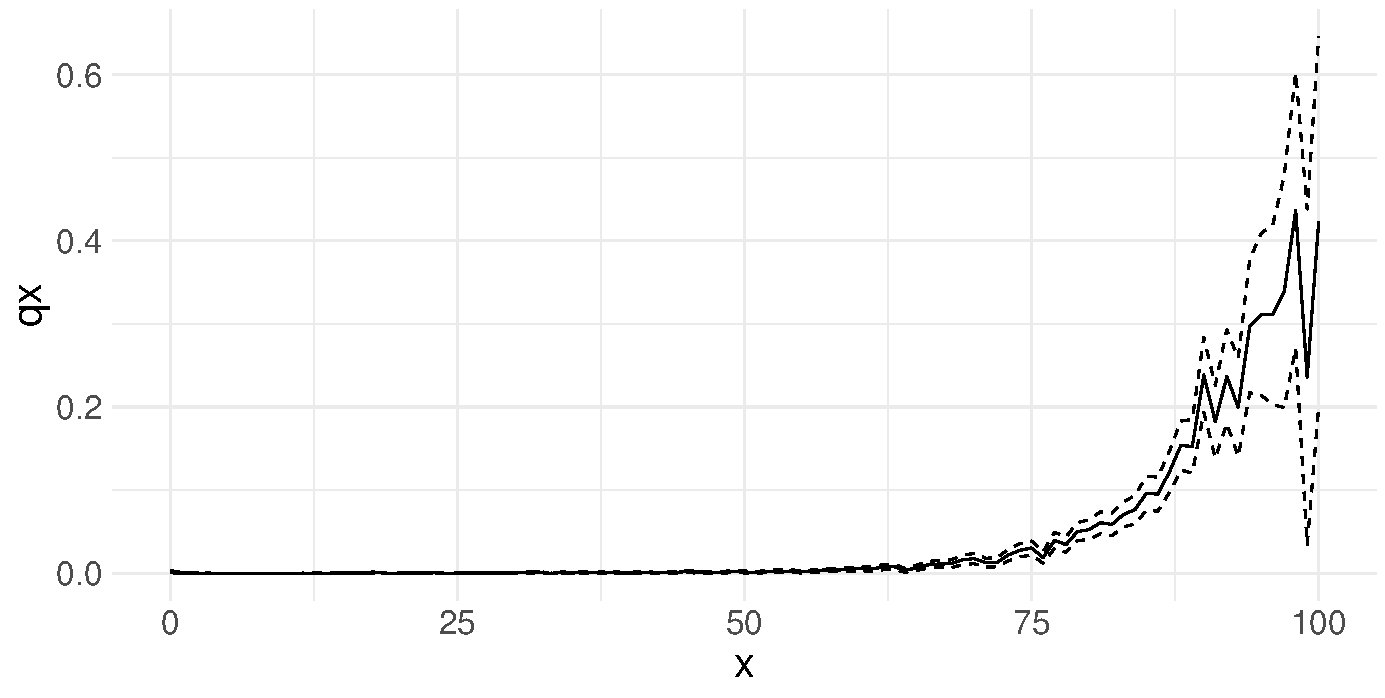
\includegraphics[width = 0.6\textwidth]{figures/qx_all}
\caption{Probabilités de décès en fonction de l'âge}
\label{qx_plot}
\end{figure}
\begin{solution}
\begin{itemize}
  \item Les lignes en pointillé correspondent à l'intervalle de confiance de la probabilité de décès (0.5 points)
  \item L'estimateur de la probabilité de décès est asymptotiquement normal (lorsque $E_x^0\rightarrow \infty$) avec 
  $$
\widehat{q}_x\sim\text{Normal}\left(q_x, \frac{\widehat{q_x}(1-\widehat{q_x})}{E^0_x}\right),
$$
on en déduit que 
$$
q_x\in\left[q_x \pm q_{1-\alpha/2}\sqrt{\frac{\widehat{q}_x(1-\widehat{q}_x)}{E_x^0}}\right],
$$
avec $q_{1-\alpha/2}$ le quantile de la loi normale d'ordre $1-\alpha/2$.
\end{itemize}
\end{solution}
\part[1] Nous décidons d'utiliser le modèle suivant 
\begin{equation}\label{eq:logit_qx}
\text{logit}(q_x) = \log\left(\frac{q_x}{1-q_x}\right) = \alpha + \beta x,\text{ }x\in\{0,\ldots, 100\}.
\end{equation}
De quelle type de procédure s'agit-il? Pourquoi utiliser une telle procédure? Votre réponse peut s'appuyer sur la Figure \ref{qx_plot}.
\begin{solution}
\begin{itemize}
\item Il s'agit d'une procédure de lissage paramétrique (0.5 point)
\item L'idée est compenser la volatilité des estimations des probabilités de décès aux grands âge due à une faible exposition. (0.5 point)
\end{itemize}
\end{solution}
\part[1] La Figure \ref{logit_qx_plot} montre le logit des probabilités de décès en fonction de l'âge.
\begin{figure}[!ht]
\centering
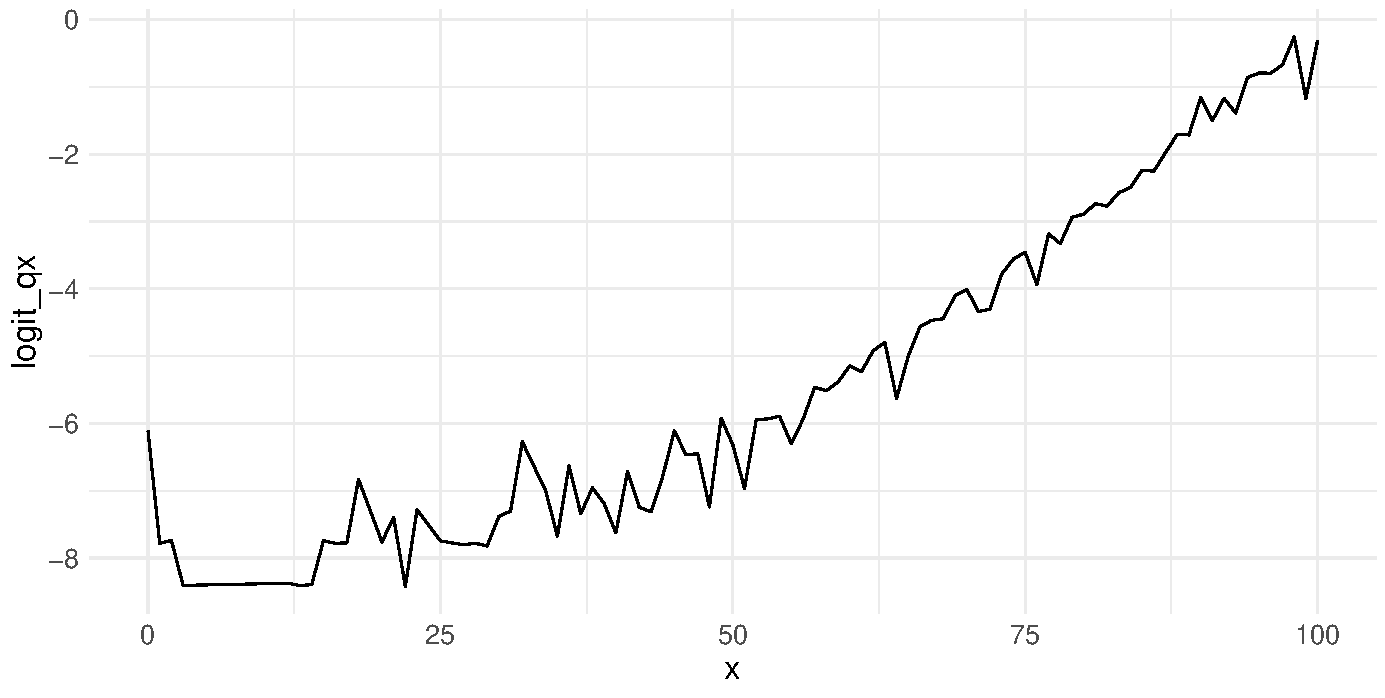
\includegraphics[width = 0.6\textwidth]{figures/logit_qx_all}
\caption{logit des probabilités de décès en fonction de l'âge}
\label{logit_qx_plot}
\end{figure}

Pensez vous que le modèle \eqref{eq:logit_qx} est adapté? Quelle information risque-t-on de rater?
\begin{solution}
\begin{itemize}
\item On note la tendance linéaire du logit des probabilités de décès en fonction de l'âge en particulier à partir de $40-50$ ans. (0.5 point)
\item On ne pourra pas capter la mortalité infantile qui risque en plus de poluer l'estimation de $\alpha$ et $\beta$. (0.5 point)
\end{itemize}
\end{solution}
\part[2] Après application de la méthode précédente, nous obtenons les probablités de décès en pointillé sur la Figure \ref{qx_smoothed_plot}. 
\begin{figure}[!ht]
\centering
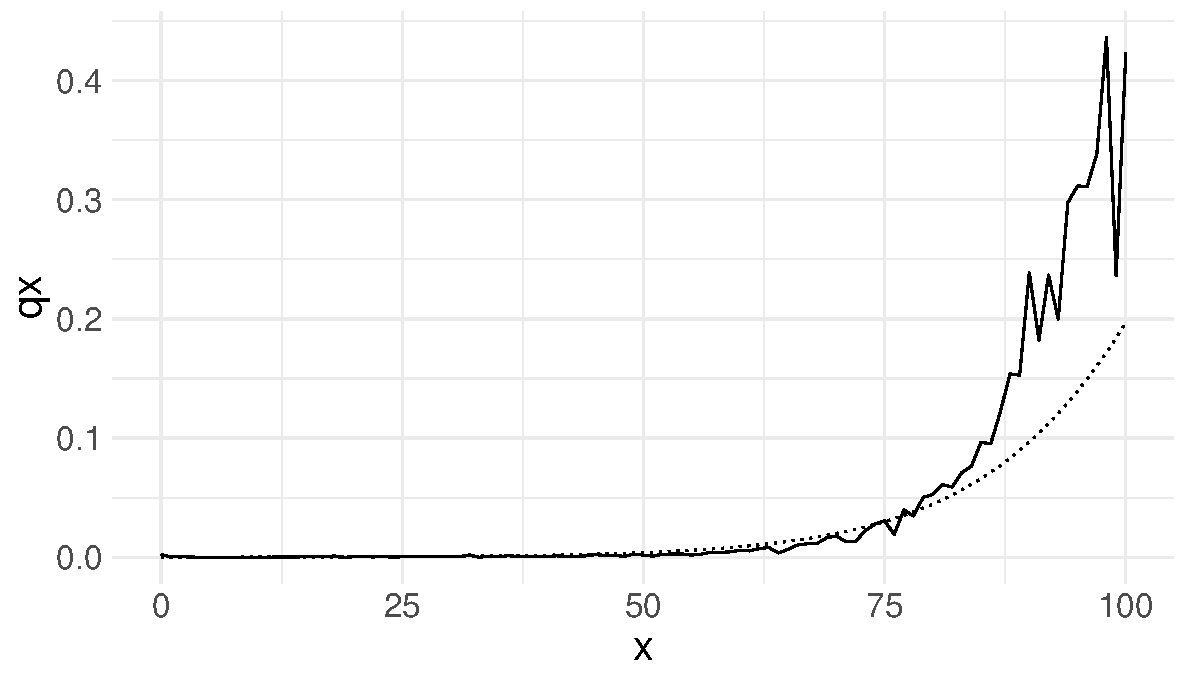
\includegraphics[width = 0.6\textwidth]{figures/qx_smoothed}
\caption{Probabilités de décès en fonction de l'âge après ajustement via le modèle logistique}
\label{qx_smoothed_plot}
\end{figure}
Que pensez-vous de cet ajustement?  Comment quantifier la qualité de l'ajustement des probabilités de décès? Comment améliorer cet ajustement? (On peut s'appuyer sur la Figure \ref{logit_qx_plot} pour justifier sa réponse).
\begin{solution}
\begin{enumerate}
\item L'ajustement est correct même si on constate une sous estimation des probabilités de décès aux grands âges. (0.5 point)
\item Il faut mesurer la fidélité des taux lissés par rapport aux taux bruts, par exemple vérifier que les taux lissés tombent dans l'intervalle de confiance des taux bruts. (0.5 points) On peut effectuer un test des signes pour vérifier qu'on ne surestime ou ne sous estime pas systématiquement les taux bruts. (0.5 point)
\item Il faudrait probablement restreindre l'interval des âges pour l'ajustement du modèle. Par exemple retirer les âges inférieurs à $40$ ans et supérieur à $80$ ans. Ce modèle logistique peut être utiliser pour extrapoler les probabilités de décès (méthode de Kannisto vu en cours). (0.5 point)
\end{enumerate}
\end{solution}
% \part[2] Les probabilités de décès pour les hommes et les femmes sont données sur la Figure \ref{qx_HF_plot}. 
% \begin{figure}[!ht]
% \centering
% 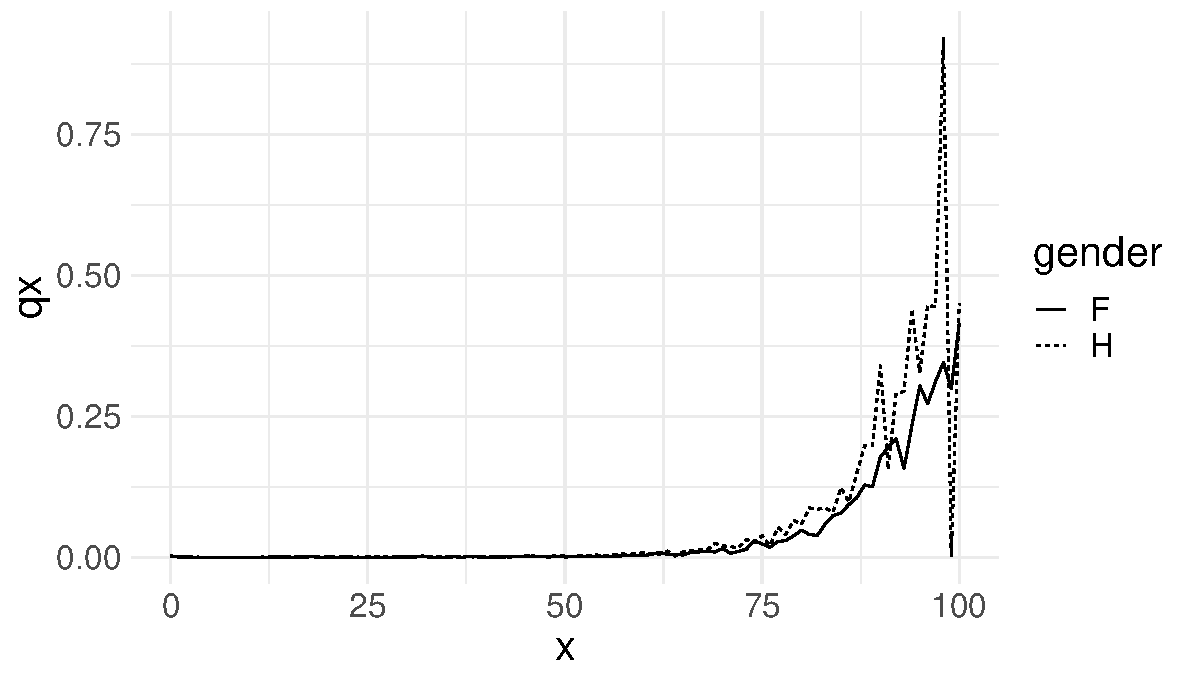
\includegraphics[width = 0.6\textwidth]{figures/qx_HF}
% \caption{Probabilités de décès en fonction de l'âge et du genre.}
% \label{qx_HF_plot}
% \end{figure}

% Comment étudier statistiquemnt la simililarité ou la différence de la mortalité entre les hommes et les femmes? Décrire la méthode.
% \begin{solution}
% La méthode à privilégier au vu des données disponibles est le test du log rang qui compare les nombres de décès observés des hommes et des femmes au nombre de décès prédit en mélangeant les deux populations. On peut recréer des nombre de décès et des exposition basés sur les probabilités de décès lissé. Une autre façon de procéder serait de comparer les résultats issus des modèles logistiques pour les hommes et les femmes. La significativité d'une variable catégorielle dans un modèle de regression va cependant au dela des notions abordés dans le cours de modèle de durée.  (1 point)
% \end{solution}
\end{parts}
\newpage
\question Nous disposons de données sur la durée des arrêts de travail dans une entreprise. Le tableau \ref{tab:data_incap} donne un aperçu des données.
\begin{table}[!ht]
\centering
\begin{tabular}{rrrrl}
  \hline
 time & status & age & gender \\ 
  \hline
5.01 &   1 &  25 & 1 \\ 
 1.14 &   0 &  50 & 0 \\ 
 7.83 &   1 &  60 & 0 \\ 
  6.75 &   1 &  25 & 1 \\ 
   5.86 &   0 &  53 & 0 \\ 
   0.27 &   1 &  55 & 1 \\ 
   \hline
\end{tabular}
\label{tab:data_incap}
\caption{Durée des arrêts de travail dans l'entreprise}
\end{table}

Les variables sont décrites ci-dessous:
\begin{itemize}
  \item \texttt{time}: Durée de l'arrêt de travail
  \item \texttt{status}: $0$= "en cours" et $1$ = "terminé". Un $0$ équivaut à une donnée censurée à droite.
  \item \texttt{age}: âge du salarié ou de la salariée
  \item \texttt{gender}: genre du salarié ou de la salariée
\end{itemize}
\begin{parts}
 \part[2] Le jeu de données est stocké sous la forme d'un \textit{data frame} nommé \texttt{df\_incap}. Nous débutons l'analyse avec le code suivant
\begin{lstlisting}
fit <- survfit(Surv(time, status) ~  gender, data = df_incap)
ggsurvplot(fit,
           pval = TRUE, conf.int = TRUE,
           ggtheme = theme_bw(), 
           linetype = "strata"
)
\end{lstlisting}
Le résultat est donné sur la Figure \ref{surv_plot_gender}.
\begin{figure}[!ht]
\centering
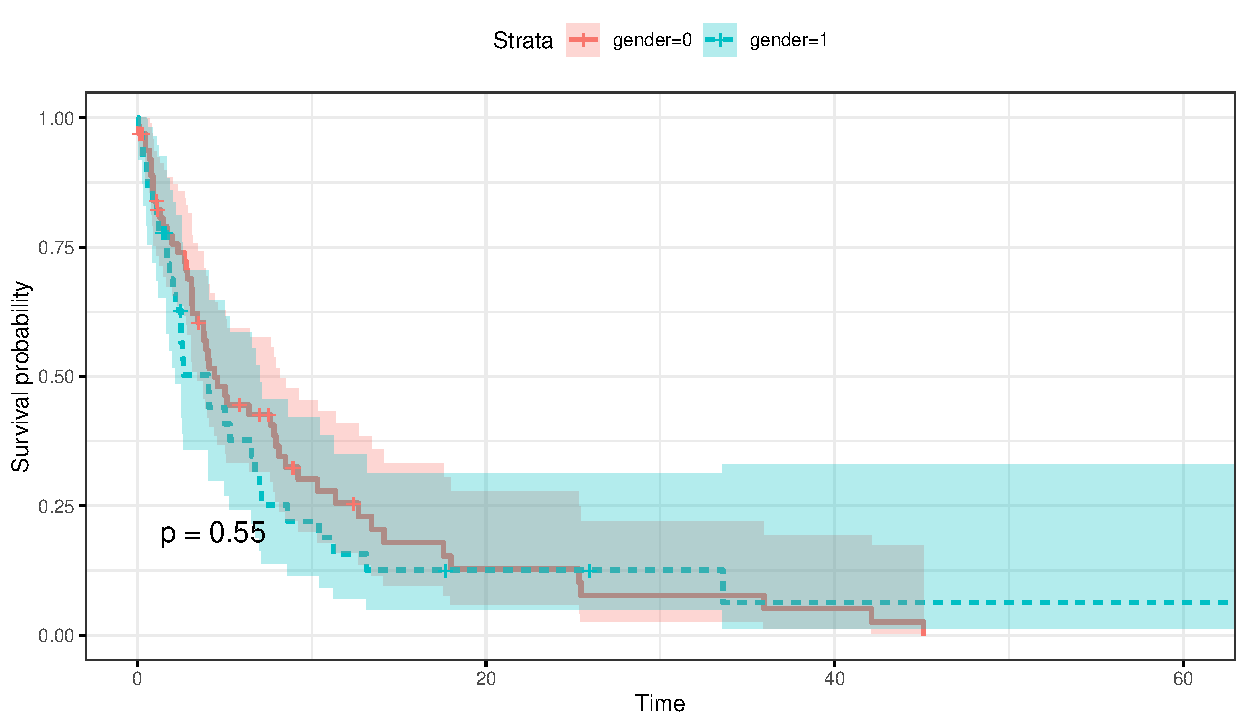
\includegraphics[width = 0.8\textwidth]{figures/surv_plot_gender}
\caption{?}
\label{surv_plot_gender}
\end{figure}
A quoi correspondent les différents éléments visibles sur le graphique? Vous devez préciser les méthodologies statistiques employées (les formules ne sont pas nécessaires) et donner votre interprétation de ce graphique. 
\begin{solution}
\begin{itemize}
  \item Nous avons les fonctions de survies de la durée des arrêts de travail au sein des populations de salariés discriminées par la variable \texttt{gender}. En présence de données censurés à droite, l'estimation est obtenue via l'estimateur de Kaplan-Meieir. La valeur estimée est entouré d'une bande qui correspond aux intervalles de confiances. (0.5 point) Nous constatons que les deux courbes de survies tombe dans l'intervalle de confiance de l'autre courbe, cela donne une indiquation quant à leur similarité statistique. (0.5 point) 
  \item L'élément $p = 0.55$ est la \textit{p-value} du test de log rang testant l'hypothèse de similarité des courbes de survie (0.5 point). Cette valeur "élevée" (supérieur à un seuil de significativité, $0.05$ par exemple) indique qu'il n'est pas possible de rejeter $H_0$ et donc qu'il n'y a pas de différence statistiquement significative entre les deux courbes (0.5 point). 
\end{itemize}
\end{solution}
\part[3] Nous poursuivons avec le code suivant
\begin{lstlisting}
res.cox <- coxph(Surv(time, status) ~ age + gender, data = df_incap)
res.cox
\end{lstlisting}
Nous obtenons dans la console le résultat de la Figure \ref{screen_shot_mdd}.
\begin{figure}[!ht]
\centering
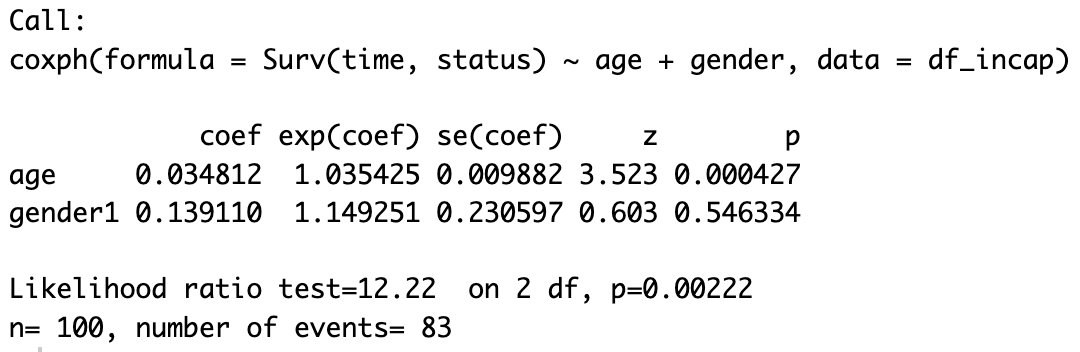
\includegraphics[width = 0.6\textwidth]{figures/screen_shot_mdd}
\caption{?}
\label{screen_shot_mdd}
\end{figure}
Quel est le modèle considéré? Rappeler les hypothèses avec une formule adaptée à l'étude de la durée des arrêts de travail considérées dans cet exercice. Quelles conclusions retirez-vous de ces résultats?
\begin{solution}
\begin{itemize}
  \item Le modèle de risque proportionel de Cox est utilisé pour analyser l'impact des covariables \texttt{age} et \texttt{gender} sur la durée des arrêts de travail (0.5 point)
  \item Le modèle de Cox définit la fonction de hasard par 
  $$
h(t) = h_0(t)\exp(\beta_1\cdot age + \beta_2\cdot\mathbb{I}_{gender  = 1})
  $$
  (1 points)
  \item La durée des arrêts de travail augmente avec l'âge car $\exp(\text{coef})>1$, de plus le test de significativité du coefficient renvoie une p-valeur très inférieure à $0.05$ (0.5 point)
  \item La durée des arrêts de travail augmente si $\text{gender} = 1$ car $\exp(\text{coef})>1$, en revanche le test de significativité du coefficient renvoie une p-valeur très supérieure à $0.05$ ce qqui indique que l'impact de la variable \text{gender} n'est pas suffisante pour être significative. Cela corrobore les résultats obtenus dans la question précédente (0.5 point)
  \item Dans son ensemble le modèle est pertinent comme l'indique le test du rapport de vraisemblance dont la pvaleur est très inférieur à $0.05$ (0.5 point)
\end{itemize} 
\end{solution}
\end{parts}
\end{questions}

\end{document}